\chapter{Background}
\label{chapter:background} 

This thesis has its foundations in \textbf{software quality assurance (SQA)} and practices building on top of it. The context of research
is based in Java-projects and testing Java-code. \textbf{Java Virtual Machine (JVM)} and its implementation in \textbf{Java Runtime Environment (JRE)}
produces the environment for Java-projects~\cite{wiki:jvm}. Therefore first in this section brief details of JVM are examined.
Before exploring the quality assurance aspects of Java-projects running on JRE (JVM), general concepts of software quality and SQA are explained.

\section{Java Virtual Machine} %1p
    JVM and its programming language Java was originally designed for building software on networked devices~\cite{lindholm2015java}. From there
    next major usage possibilities for Java came from Web HTML-sites. Web-sites with Java embedded programs first appeared in HotJava-browser~\cite{lindholm2015java}.
    From those days usage of Java has explored new fields and JVM itself hosts nowadays many more programming languages than
    just Java~\cite{wiki:jvm}.

    JVM is an \textbf{abstract computing machine} that provides instruction set and different memory areas at runtime.
    Current implementations of JVM have brought the environment to mobile, desktop and server devices, yet the JVM itself
    isn't tied to any specific technology. The basic information for JVM comes from \textit{class} files. These files include
    binary JVM bytecode instructions. Instead of having Java code in class files, it compiles to these binary instructions
    that are run on JVM. Figure \ref{fig:JVM} illustrates the runtime memory areas and the class loader system.
    JVM has support for \textit{primitive} and \textit{reference} types, from which latter enables support for referencing JVM objects. ~\cite{lindholm2015java}

    JVM is interesting target for a vast amount of programming languages, thanks to its maturity, ubiquity and performance~\cite{sarimbekov2013characteristics}.
    These programming languages pass as a valid JVM language if their functionality can be expressed in a valid class file~\cite{wiki:jvm}.
    Programs written in ported dynamic languages such as \textit{Ruby (JRuby)} or \textit{Python (Jython)}~\cite{sarimbekov2013characteristics} can be run on the JVM.
    JVM also hosts an array of new programming languages such as \textit{Scala, Clojure} and \textit{Groovy}~\cite{wiki:jvm}.

    The possibilities of these additional JVM programming languages are crucial part of this thesis. Later on testing Java-code is examined with
    different implementation level \textbf{Behavior Driven Development (BDD)} -frameworks from various JVM languages.

    \begin{figure}[ht]
      \begin{center}
        \includegraphics[width=12cm]{images/jvm.png}
        \caption{Overview of internal architecture of Java Virtual Machine}
        \label{fig:JVM}
      \end{center}
    \end{figure}

    \clearpage

\section{Software quality assurance}
    The standard definition of quality assurance states it to be:
        \textit{"A planned and systematic pattern
        of all actions necessary to provide adequate confidence
        that the item or product conforms to established
        technical requirements"}.~\cite{buckley1978standard}
    Although modern software quality assurance differs from the original standard definition, it is still definitely found
    at the core of SQA. To fully understand SQA and why it is important, first the software quality concept in itself is illustrated.
    Motivation for practicing SQA is examined second and third the overall activities in SQA are explained briefly.
    \subsection{Definitions of quality}
    Quality in software development is a multifaceted entity that has had many viewpoints for a long time.
    Some of these earlier views include \textit{product, transcendental, user, manufacturing} and \textit{value based} view~\cite{kitchenham1996elusive}.
    Because there exists so many viewpoints to what software quality is, it makes the measuring of quality hard~\cite{kitchenham1996elusive}.
    Business goals and their priorities should determine the needed level of software quality~\cite{kitchenham1996elusive} so therefore
    quality in itself is not set in stone, but it can alter between software services and products to fit the purpose.
    This can be easily demonstrated with an example of software inside a missile defence system or an online dating application.
    Two different systems with different goals and consequences of use and therefore obviously different standards for needed quality.

    \begin{figure}[ht]
      \begin{center}
        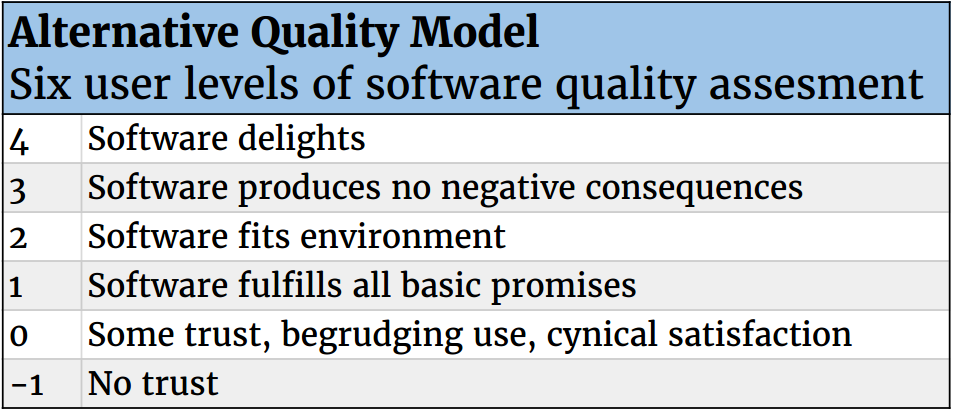
\includegraphics[width=10cm]{images/alternativeQM.png}
        \caption{Alternative Quality Model}
        \label{fig:AQM}
      \end{center}
    \end{figure}

    New alternative view on software quality by Denning~\cite{denning2016sq} includes user experience directly in the core of quality.
    This view is called the \textbf{alternative quality model (AQM)} and it defines quality software as software that delights
    the end user~\cite{denning2016sq}. Figure \ref{fig:AQM} displays the full scale of AQM.
    In my opinion, this view on software quality has strong correlation to customer value. Customer value can be seen as
    the benefits and sacrifices the end user experiences using the product~\cite{woodruff1997customer}. Therefore traditional
    defect free software quality is an important part of providing end user with software that delights, as defects
    can be seen as sacrifices that devour the trust towards software. Nevertheless this is not the only part of AQM,
    but providing software that delights the end user needs to also solve the right problem for the user.
    Thus software quality on the AQM is almost directly linked to customer value; it needs to be defect free but also
    provide benefits in use to delight the end user. While this research is mainly interested in aspects of producing traditional defect free quality software,
    later on in this chapter BDD is examined in detail. BDD can be seen to directly try to increase software quality on the AQM.

    \subsection{Motivation for SQA}
    Many software projects fail but also many of them are successful. Success and failure in this context have multidimensional meaning with
    \textit{technical, economic, behavioral, psychological} and \textit{political} aspects ~\cite{mcleod2011factors}. Aggressive
    schedule can be usually seen as one of the primary causes for software project failure~\cite{cerpa2009did}. This can cause
    problems on many of the projects multidimensional axis, for instance in technical- and economical aspects. Projects might go
    over the budget, schedule, not meet the user needs and eventually be released with low quality ~\cite{cerpa2009did}.
    Although many of the problems are related to requirements engineering \textbf{(RE)}, a lot of them are fixes or rework needed after launch~\cite{lessons}.
    If quality is measured on the AQM, then both RE and SQA are intertwined in the concept of software quality and SQA-work
    is essential for the success of software project. Even if software quality is only limited to mean defect free software, SQA has
    major role in preventing project failures.

    \subsection{Activities in SQA}
    Quality assurance practices and activities differ greatly in rhythm and also to a lesser degree in practices used in
    traditional waterfall-model software projects vs agile projects~\cite{huo2004software}. Waterfall-projects have a rule set
    of their own for quality assurance, but for the topic of thesis agile methodologies and their SQA-practices are more relevant.
    SQA-practices can be generally categorized to \textit{defect detection, code enhancement, verification \& validation (V\&V)} of artifacts,
    and \textit{collaboration \& communication} between stakeholders.

    Defect detection can be split into two categories: \textbf{explicit} and \textbf{implicit} defect detection activities~\cite{mantyla2014software}.
    Implicit defect detection means finding defects as a secondary result when the goal was to perform another activity,
    such as demo presentation or giving training about the software use~\cite{mantyla2014software}. Explicit defect detection activities
    hold ones such as \textit{testing} and artifact \textit{inspection}, but they are found to have a lower
    defect detection rate than implicit ones~\cite{mantyla2014software}. \textit{Continuous integration} can also be seen
    as a explicit defect detection as it illustrates integration defects and problems with frequent integration cycle~\cite{huo2004software}.

    Code enhancement activities aim to produce better design and maintainability of the codebase and these include practices
    like \textit{pair programming, refactoring}~\cite{huo2004software} and \textit{code reviews}~\cite{rigby2013convergent}.
    Although code reviews are also a form of inspection and explicit defect detection, one of their primary uses in modern
    code review is to share knowledge between team members~\cite{mantyla2014software}~\cite{rigby2013convergent}.

    Verification \& Validation aims to guarantee the quality of product or intermediate products and it can be used for
    example to design and requirement artifacts. It is a static method, which involves stakeholder(s)
    inspecting the artifact. It is more of a traditional waterfall software project activity, but agile practices such as code reviews
    can be categorized as a V\&V activity. ~\cite{huo2004software}

    Collaboration and communication between stakeholders are used in agile methodologies frequently being one of the
    cornerstones of agile practices in general~\cite{huo2004software}. Frequent customer collaboration with \textit{On-site customer}~\cite{huo2004software}
    is an agile SQA-practice that establishes a foundation for many agile practices and is essential in delivering
    quality on the AQM.

    There are many more specific SQA practices that have their foundations on the activities mentioned in this section.
    Next in this thesis testing is examined in detail through automated testing as it provides a base for \textbf{Test Driven Development (TDD)}
    and BDD.

\section{Automated testing}
    First in this section different levels of test automation are explored. Second lower levels of test automation are explained in more
    detail and third overall benefits and drawbacks of test automation are discussed.

    \subsection{Levels of automation}
    \begin{figure}[ht]
      \begin{center}
        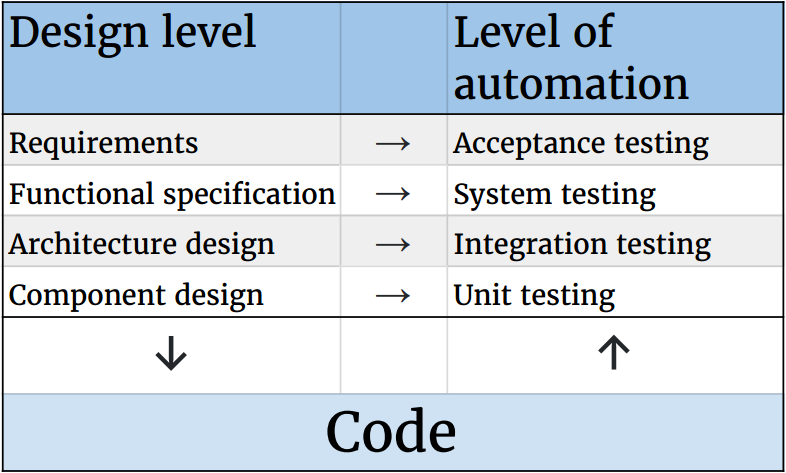
\includegraphics[width=10cm]{images/testlevels.png}
        \caption{Test last development regarding system and its design}
        \label{fig:testlevels}
      \end{center}
    \end{figure}

    Test automation comes at many levels of granularity regarding the system and its requirements. The four main levels for
    functional testing are \textit{unit, integration, system} and \textit{acceptance} testing~\cite{itkonen2016}.
    Figure \ref{fig:testlevels} illustrates how different levels of design relate to levels of test automation in traditional
    \textbf{Test Last Development (TLD)}. At the bottom
    of figure \ref{fig:testlevels} there is code, which is the result of design and foundation (in traditional automated testing)
    for different testing levels. Different levels of design guide the automated tests at the specified level.

    The introduced test automation levels are a part of functional testing. There exists also different non-functional
    requirements for software projects that can be automatically tested, such as \textit{performance} and \textit{security} testing~\cite{crispin2009agile}.
    These are not in the scope of this study, instead the functional testing levels of automated unit and integration testing are
    the main topic of interest.

    \subsection{Low level testing explained}
    Low level testing in the scope of this thesis means automated unit and integration level testing. They both have separate
    definitions and usages inside software projects, but the distinction between the two can be found confusing by many developers~\cite{artofunit2013}.
    Figure \ref{fig:testlevels} illustrates how unit testing adheres to component design and integration testing to architecture design ~\cite{itkonen2016}.

    \textbf{Unit test} has many similar definitions which all agree that it tests individual unit or collection of these units working as one
    ~\cite{runeson2006survey}~\cite{whittaker2000software}. Unit test also has the property of being isolated from the rest
    of the system~\cite{whittaker2000software}. Unit testing can in a sense also be seen as an intersection of design,
    coding and debugging~\cite{langr2015pragmatic}.
    Dedicated practitioner of unit testing Osherove~\cite{artofunit2013} has identified important aspects of a good unit test:
    \textit{trustworthiness, maintainability, readability, isolated,} has \textit{single concern} and contains \textit{minimal repetition}.

    \textbf{Isolation} is an important part of unit testing. This means in practice using test doubles also known as \textit{mocks}.
    Using mocks in unit tests means substituting real objects with limited functionality provided by mocks. Mocks can be
    configured to behave always in a specified manner. This configured behavior of mocks is called \textit{stubbing},
    in which output result of mock object can be injected from the test code. Traditional uses of mocks are for instance using
    them to make progress without implementing dependencies (used in TDD/BDD), isolating unit under test from dependencies
    or nondeterminism. ~\cite{chelimsky2010rspec}

    \textbf{Integration testing} is the second, higher level of automated testing in the low level testing scope of thesis.
    The definitions of integration testing state that it is a testing
    activity which involves multiple components~\cite{whittaker2000software}~\cite{artofunit2013}. Osherove~\cite{artofunit2013}
    defines integration testing as testing a unit of work with real dependencies in place, for instance database and  networking.
    Integration tests are not usually as fasts as unit tests~\cite{artofunit2013}. Many times this results from including
    full context of the system through dependency injection container, such as \textit{Spring Framework} or \textit{Guice}~\cite{kapelonis2016java}.

    \subsection{Benefits and drawbacks of automated testing}
    Agile methodologies do not prefer or deny separate testers inside a project, but for a modern quality centered
    development separate testers might hinder the experience~\cite{prechelt2016quality}. Teams without separate testers have one aspect in common,
    they rely heavily on test automation as the core of quality. One of the most important properties in these kind of
    teams is the rapid and direct feedback that test automation can provide~\cite{prechelt2016quality}. Overall the task of test automation
    doesn't come with benefits only, but it has also its drawbacks.

    \textbf{Benefits} of test automation are vast. Systematic literature review by Rafi et al.~\cite{rafi2012benefits} has found many
    of them through various sources. Some of them can be highlighted: \textit{improved product quality, test coverage increase,
    increase in developer confidence} and \textit{reduced testing time}~\cite{rafi2012benefits}.

    Automated testing was found also to allow \textit{shorter release cycles}. This is a result of
    tests executed more often and therefore allowing defects to be detected earlier with reduced cost to fix.
    Quality and depth of test cases also increase with automation, as less time is needed for executing them and more time is available
    to design the test cases. Another benefit of automated testing is the more layered, testable design of the software.
    To achieve the \textbf{benefits}, test automation \textbf{strategy needs to combine different approaches} and testing levels. ~\cite{berner2005observations}

    Automated test cases can also \textbf{help to understand} the system. This is enabled by writing information how the production code should behave
    into the test cases and test methods. ~\cite{langr2015pragmatic}~\cite{chelimsky2010rspec}~\cite{kapelonis2016java}

    At unit testing level, benefits of test automation was found to include over 20\% decrease in test defects~\cite{williams2009effectiveness}.
    Also the defects found by largely increased customer base in first 2 years of use was decreased by introducing unit testing practices~\cite{williams2009effectiveness}.
    Another strength of automated unit testing is also the continuous regression suite it provides~\cite{runeson2006survey}.

    Unfortunately test automation isn't only beneficial compared to manual testing. In the earlier mentioned review by Rafi et al.~\cite{rafi2012benefits}
    some of the \textbf{limitations} include for instance: \textit{automation can't replace manual testing, difficulty in maintaining}
    and \textit{lack of skilled people} for test automation. Usually the lack of skilled people tends to result in projects as
    \textit{inapporiate test automation strategies}~\cite{rafi2012benefits}~\cite{berner2005observations}. These kind of projects
    usually automate testing at wrong levels, for instance automatically testing through Graphical User Interface (GUI). This
    can lead to brittle tests that are hard to maintain as the GUI changes~\cite{berner2005observations}. Neglecting automated
    testing maintenance can lead to knowledge diminishing and tests that lose totally their capability to run~\cite{berner2005observations}.
    Altogether testware maintenance is hard and this can be many times seen as tests that are not engineered
    with the same attention to detail as actual production code~\cite{berner2005observations}.

    At unit testing level, drawbacks of test automation include approximately 30\% more development time compared to manual testing~\cite{williams2009effectiveness}.
    Runeson~\cite{runeson2006survey} also found unit testing drawbacks similar to the afore mentioned automated testing problems by other studies.
    These include \textit{unit testing of GUI}, \textit{competency of developers} working with unit tests and \textit{unit test maintenance}~\cite{runeson2006survey} .
    Also the cost of unit test versus the value it provides was found problematic amongst unit testing practitioners~\cite{runeson2006survey}.

\section{xUnit testing frameworks} %2p
    xUnit family of testing frameworks are free, open source software for various programming languages that
    all share the same basic architecture. The first implementation of a xUnit test framework was \textit{SUnit}
    for Smalltalk in 1999.  From there the same idea was ported for Java and thus \textit{JUnit} was born. There exists also many other
    xUnit family members, for instance \textit{CppUnit} for C++, \textit{NUnit} for .NET languages and \textit{PyUnit} for Python.
    These unit testing frameworks are extensible with different types of extensions. Extensions can add for example integration testing capabilities
    for different domains. ~\cite{hamill2004unit}

    This thesis is interested in developer practices with JUnit and their perception towards it, therefore next the xUnit family architecture
    is examined with JUnit. After architecture, a closer look is taken to see how JUnit can be extended for Spring Framework
    integration testing.

    \subsection{JUnit}
    JUnit acts as the reference implementation of the xUnit family and it is also the most popular instance of them~\cite{hamill2004unit}.
    It is used for Java-code testing and it can be extended for many domains in Java testing~\cite{hamill2004unit}.
    Current stable version of JUnit is \textit{JUnit4}~\cite{junit4}, but \textit{JUnit5} is scheduled to release in Q5 of 2017~\cite{junit5schedule}
    providing many new features for Java testing. The examples of JUnit and empirical research in this thesis are all based on JUnit4.

    \begin{figure}[ht]
      \begin{center}
        \includegraphics[width=13cm]{images/junit.png}
        \caption{JUnit architecture}
        \label{fig:junit}
      \end{center}
    \end{figure}

    The basic architecture of JUnit consists of classes \textit{TestCase, TestRunner, TestFixture, TestSuite} and \textit{TestResult}.
    \textbf{TestCase} is the unit test base class, that holds runnable \textbf{test methods}.
    It implements the interface \textbf{Test} and its \textit{run()}-method. Test methods use \textbf{assertions} inside them to evaluate test conditions.
    \textbf{TestRunner} class is for extending JUnit and running multiple test cases at once and reporting
    them. \textbf{TestFixture} class is used to ensure test isolation and creating a separate test environment for each test method.
    TestFixtures provide a common shared context for test methods, but the environment is created from scratch for each test.
    This is enabled by providing the test case with common setup and teardown functionality for class and method level.
    \textbf{TestSuite} is a class made for grouping TestCases and it also implements Test. TestSuite makes it possible to run multiple TestCases and can
    be used with TestRunner. \textbf{TestResult} class is used to collect test method outcomes from TestSuites and TestCases.
    Figure \ref{fig:junit} visualizes the relationships between the core classes, interfaces and methods of JUnit architecture. ~\cite{hamill2004unit}

    \subsection{Extending JUnit for Spring Framework domain}
    \textbf{Spring} is a framework for Java, described as:
    \textit{"core support for dependency injection, transaction management, web applications, data access, messaging, testing and more."}~\cite{spring}
    It is targeted for Java enterprise applications, providing teams with a framework that allows them to primarily focus on
    application's business logic~\cite{spring}. Spring framework ships with a lot modules and features that needs to be
    configured for the project~\cite{wiki:spring}. \textbf{Spring Boot} is \textit{convention-over-configuration} solution
    composed of the Spring Framework components, that enables rapid application development with minimal effort to get started~\cite{wiki:spring}.

    Spring Framework integration testing can be done by extending JUnit with custom Spring JUnit runner class or by using Spring JUnit class and
    method rules. Runner class and the Spring JUnit rules both provide standard Spring test context
    for integration tests with features such as dependency injection and transactional test method execution. ~\cite{springintegration}

    \begin{figure}[ht]
      \begin{center}
        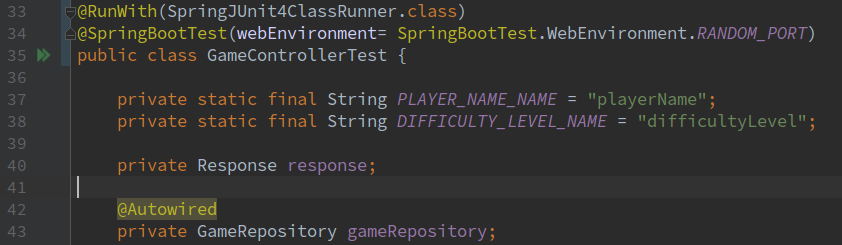
\includegraphics[width=13.5cm]{images/springrunner.png}
        \caption{JUnit extended for Spring integration testing}
        \label{fig:springrunner}
      \end{center}
    \end{figure}

    Figure \ref{fig:springrunner} shows example of a Spring Boot JUnit integration test, where the context and its configuration are
    loaded with lines 33 and 34. Line 33. is an example of extending JUnit with custom runner. Lines 42-43 show example of injected dependency
    via Spring Framework.

    JUnit and its extensions provide a base for automated low level testing of Java-code.
    Next in this thesis, before examing alternatives for low level testing of Java-projects, agile methodologies Test Driven Development
    and Behavior Driven Development are reviewed.

\section{Test Driven Development} %2p
    \subsection{Definition}
    \subsection{Benefits and drawbacks}

\section{Behavior Driven Development} %2p
    \subsection{Definition}
    \subsection{BDD vs TDD}
    \subsection{Levels of specification}
    \subsection{Tools}
    \subsection{Benefits and drawbacks}
\section{Behavior Driven low level testing frameworks} % 5p
    \subsection{Spec family}
            -Rspec and Spectrum\newline
            -Rspec / BDD Helps to shift viewpoint from 1-1 relationship between test-code and only one test method per function
    \subsection{Spock}
\section{Related research} % 2p
    -Analysis of problems found from automated testing surveys\newline
    -Reference to future research introduced in thesis work\newline

    Dippatyöstä TOWARDS AN EMPIRICAL EVALUATION
                OF BEHAVIOUR - DRIVEN DEVELOPMENT\newline
    -Suora lainaus: The benefits of developing a system written in a static language such as Java, while specifying its
     behaviours using a more flexible dynamic language such as JRuby could be analyzed.\newline\newline

    A Survey on Unit Testing Practices and Problems:\newline
    -Developers are striving to find realistic scenarios.\newline
    -Isolating unit under test was found hard (mocking etc)\newline
    -There clearly is potential for unit testing research to help developers produce better tests that make debugging and fixing easier\newline
    -Understanding code is bigger problem than understanding test code\newline
    --> If good tests can be generated, then these may help in understanding the code.\newline
    -Only half of the respondents enjoy writing unit tests\newline
    --> There is a need for tools that rise the enjoyment\newline
    -Maintaining unit tests is found harder than writing unit tests\newline
    --> Need for easier maintaining. Can better readability, Easy parametrization and code repetition removal practices help?\newline\newline

    Automatically Documenting Unit Test Cases:\newline
    -Majority of developers (60.38percent) found understanding of unit test cases to be at least moderately difficult\newline
    -Developers find up-to-date documentation and comments within test cases to be useful\newline
    -Writing comments to unit tests is a practice rarely or never done\newline
    -In order to effectively maintain test cases, it is important that developers understand the impact of each unit
     test case and the particular functionality that it aims to test.\newline
    -Developers feel that tests should be self-documentating\newline
    -More than half of the developers indicated a difficulty of moderate to very hard in terms of understanding unit tests.\newline
    -Emphasizing this importance, we observed that 89.15percent of developers agree or strongly agree that maintaining test cases
      impacts the quality of the system. This suggests that developers could benefit from tools that support them in maintaining unit test
       cases during software evolution and maintenance\newline\newline

   Tsiigaa myos Berner ja testware maintenance problems~\cite{berner2005observations}

   Per Runeson: A Survey of Unit Testing Practices\newline
   -Unit tests are documented in test code rather than in text\newline
   -Unit test motivation in agile: test suites could function as a specification\newline
   -Maintaining was found to take much effort\newline
   -Developer motivation working with unit tests needs improvement\newline
\section{Research hypothesis} %1p
    Discussion about research hypothesis (BD-testing vs JUnit) and how it relates to problems found (8) and benefits mentioned in section 6-7.\newline
    -Developers will write more granular test cases\newline
        %-Ubiquitous language
        %-BDD Helps to shift viewpoint from 1-1 relationship between test-code and only one test method per function
    -Developers will find easier to understand test cases\newline
        %-More comments, longer descriptions naturally in use through ubiquitous language
        %-Test Code should describe the behaviors of the object
    -Developers will find it easier to maintain code\newline
         %-Test Code should be part of system’s documentation
         %-Test Code should have less repetition
    -Developers will perceive working with low level automated testing more enjoyable\newline
